\chapter{Design and implementation}
As it was previously decided to create some graphical interface for the interactive installation, using Unity, some considerations was to be made in regards to the layout. This chapter will focus on the decisions made, to create a smooth interface and a good user experience. In order to create a smooth interface that would excite people in using the setup at the library, a background, some character and some interaction was to be made.

\section{The graphical layout}
\subsection{Drawing the scene}
The first step into developing a good-looking set was to develop a suitable background that ultimately would create a Christmas-like mood. The original idea was to have a few different sets to choose from, depending on the time of the day or week. However initially one background was created to run the prototype testing on. The first background created consist of a static winter landscape, together with some dynamic movable trees which will be described later.\\
In addition; due to light conditions at the library the colors chosen for the background are not all bright, but slightly soften. This action was taken in order for the projector to output a usable illustration. The scene is illustrated on  figure \eqref{fig:ip_Background}.

\begin{figure}[htbp]
\centering
\includegraphics[width=1.00\textwidth]{Pictures/Design/Background.png}
\caption{Image illustrating the initial background for the Christmas game}
\label{fig:ip_Background}
\end{figure}

\subsection{Additions to the scene}
To make the background even more interesting some extra features are implemented. As mentioned above the main idea was to have different backgrounds which changed in a given time interval. Since this wasn't made for the prototype, a sun was implemented instead. The sun start from the left side, and moves during the day till it in the end goes down in the right side. The higher the sun is placed, the more light - which gives the user the possibility to visit two different times and see different backgrounds. Another addition is larger Christmas trees, with Christmas balls or bells on them. The biggest tree even has a star on top which sparkles. \\
Last but definitely not least Santa will appear in top of the scene in his sleigh with his reindeer's. Santa will appear once in a time interval of 1-59 minutes. When he appear the timer will reset, and he will show up again in between 1-59 minutes. In theory he could show up every minute, but in average he should appear every half hour. The reason for the interval is to make his appearance special and interesting. When Santa appears sounds of bells will come and the users will hear his known laugh: "Ho-ho-ho". Furthermore he will drop presents which the users can interact with.

\subsection{Avatars}
In addition to the background created for the illustration at the library, some avatars were to be made. Considerations towards creating suitable avatars were made and it was decided to create a pixie boy- and girl, a snowman, an angle and a squirrel.
\subsection{Self-drawn}
It was decided to draw the avatars by hand instead of using some premade drawings from the internet. The avatars should then be imported as assets in Unity. \\
To start with outlines of the characters was drawn on sheets of paper. When the outlines was satisfying they were imported to the computer and drawn again inside Photoshop using drawing tablets. The drawing tablets has pressure sensor which makes the lines thickness chance accordingly to how hard you push. This brings life into the characters and makes them more interesting to look at. At last the characters was coloured, to make a bigger contrast to the background, and to make it more appealing to the audience.\\
Considering the primary group of people trespassing the setup at the library, it was decided to give the avatars a cartoonish look. This was done by using a variety of techniques. One of them was to create oversized body parts e.g. oversized heads. Two of the characters; a pixie girl and an angel is shown on figure \eqref{fig:PixieGirl} and \eqref{fig:Angel}

\begin{figure}[htbp] \centering
\begin{minipage}[b]{0.45\textwidth} \centering
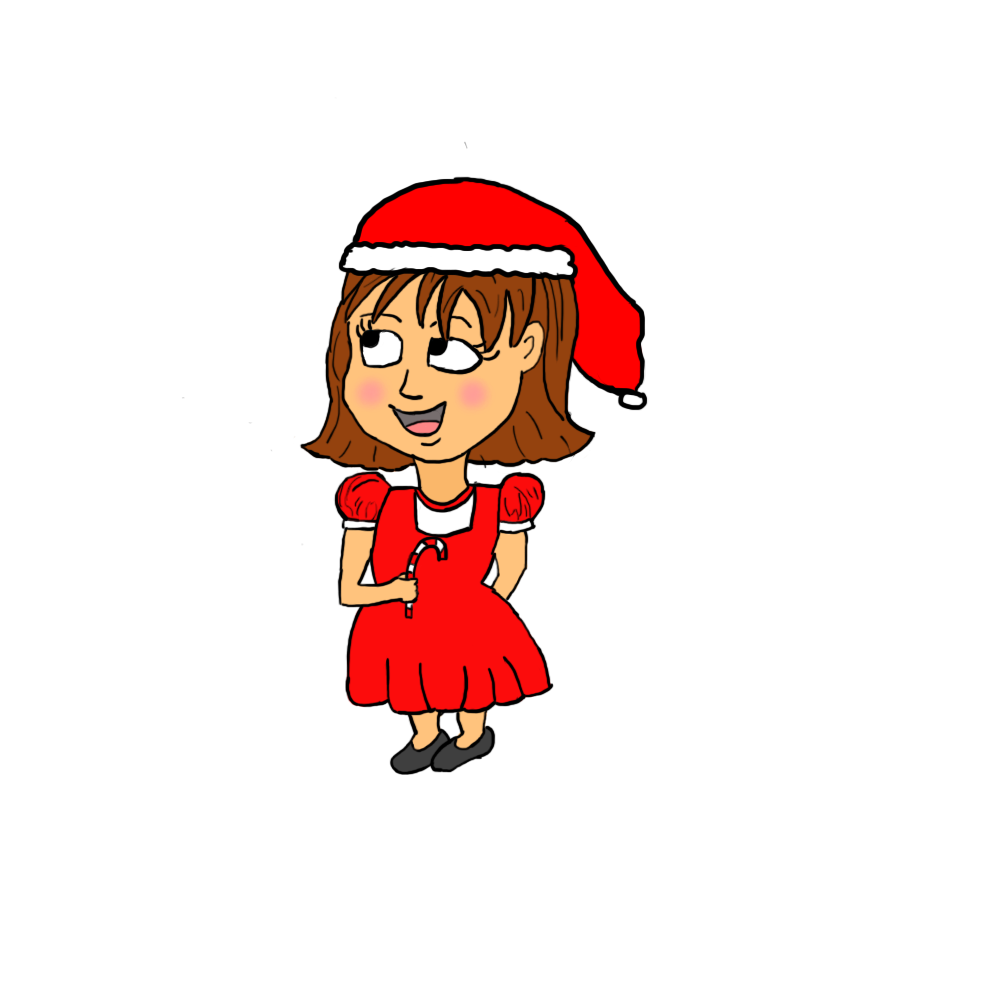
\includegraphics[width=1.00\textwidth]{Pictures/Design/PixieGirl} % Venstre billede
\end{minipage} \hfill
\begin{minipage}[b]{0.45\textwidth} \centering
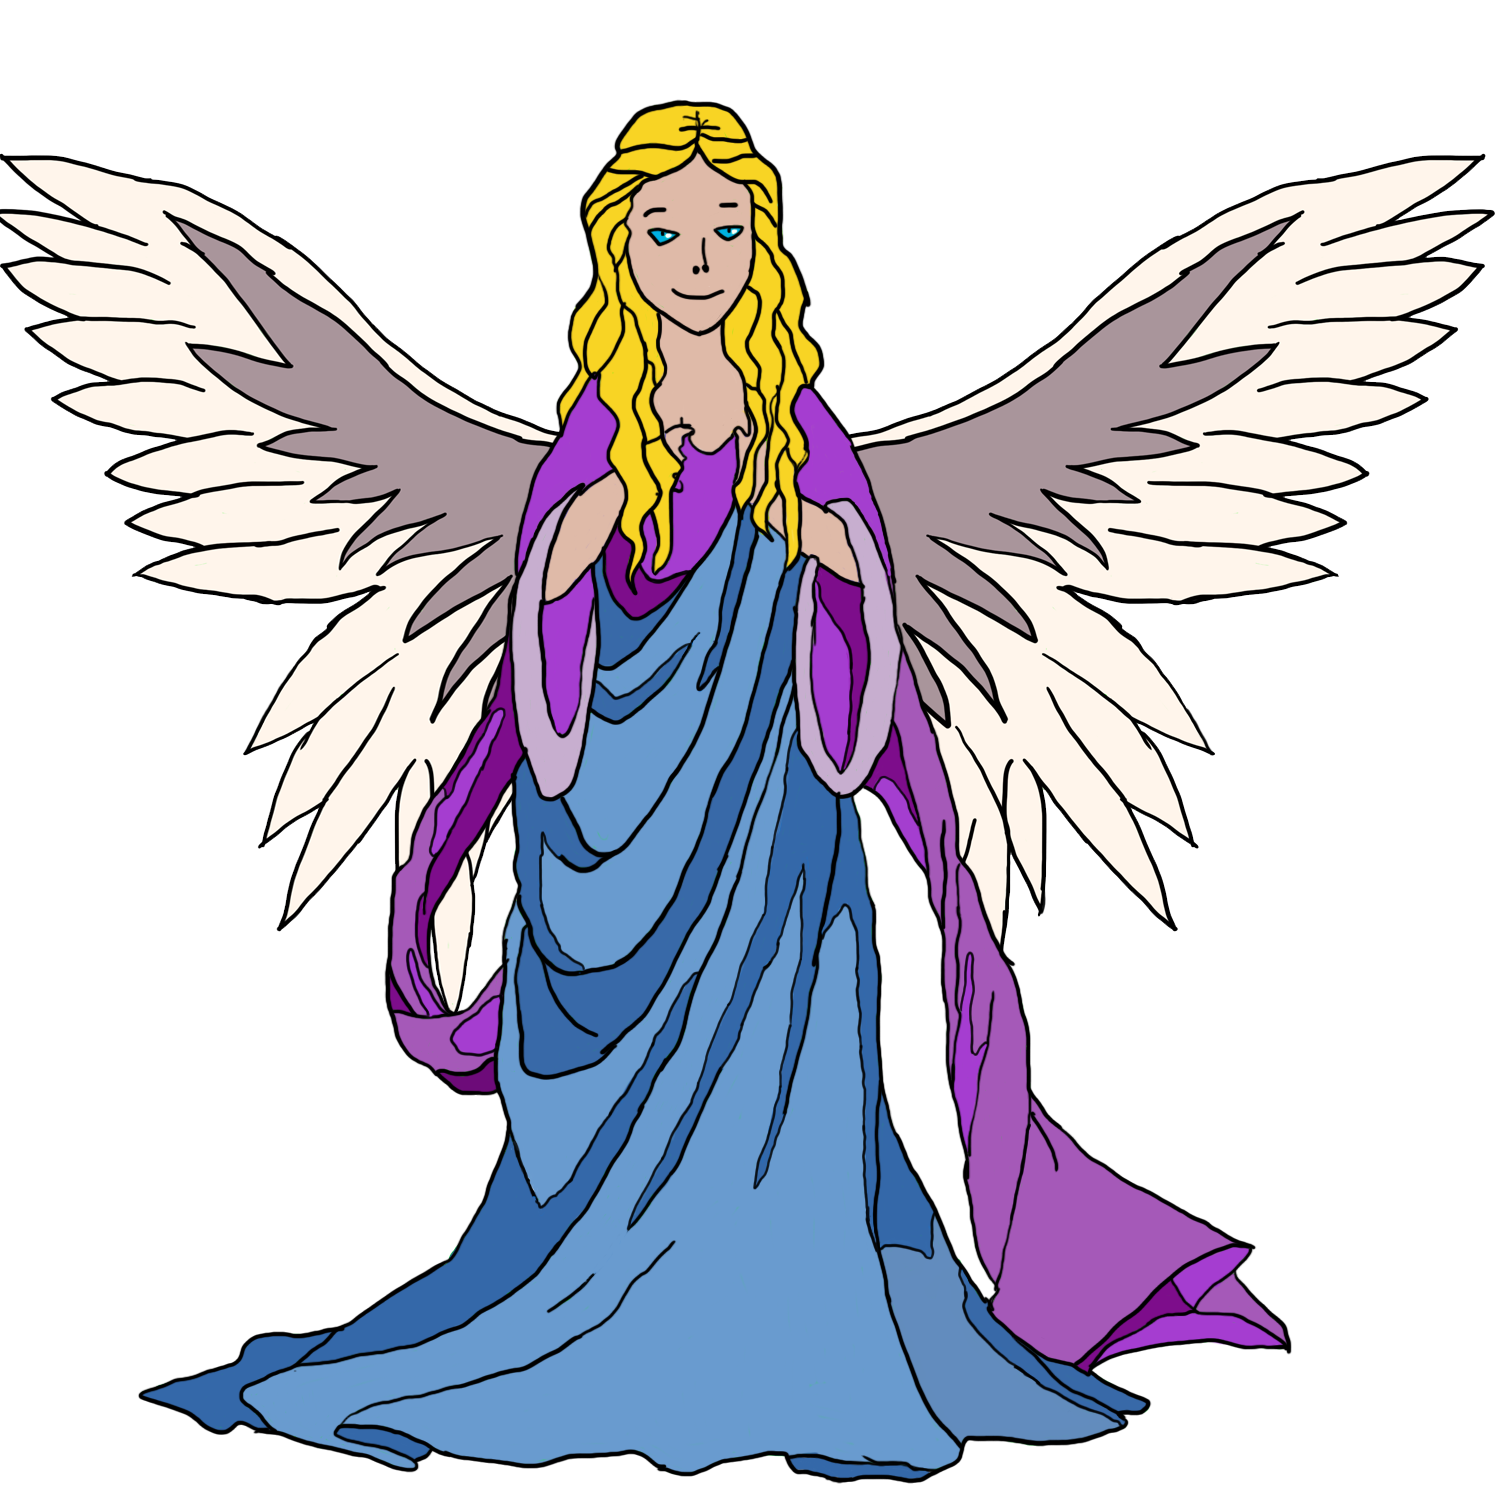
\includegraphics[width=1.00\textwidth]{Pictures/Design/Angel} % Højre billede
\end{minipage} \\ % Captions og labels
\begin{minipage}[t]{0.45\textwidth}
\caption{Pixie Girl Avatar} % Venstre caption og label
\label{fig:PixieGirl}
\end{minipage} \hfill
\begin{minipage}[t]{0.45\textwidth}
\caption{Angel Avatar} % Højre caption og label
\label{fig:Angel}
\end{minipage}
\end{figure}

\subsection{Animations and why}
In order to create some excitement towards the game; animations were added, as static scenery/avatars tend to bore the user. It was decided to give the avatars some animations for each movement. In practic 3 animations were created. There would be a primary stance if the user would stand still and a movement simulating a walk cycle if the user would move to either the right or left. The horizontal movement was however mirrored so going left and right will produce the same animation only inverted.
Figure \eqref{fig:Design_SnowmanAnimation} illustrates the three different animations made for one of the avatars.
\begin{figure}[htbp]
\centering
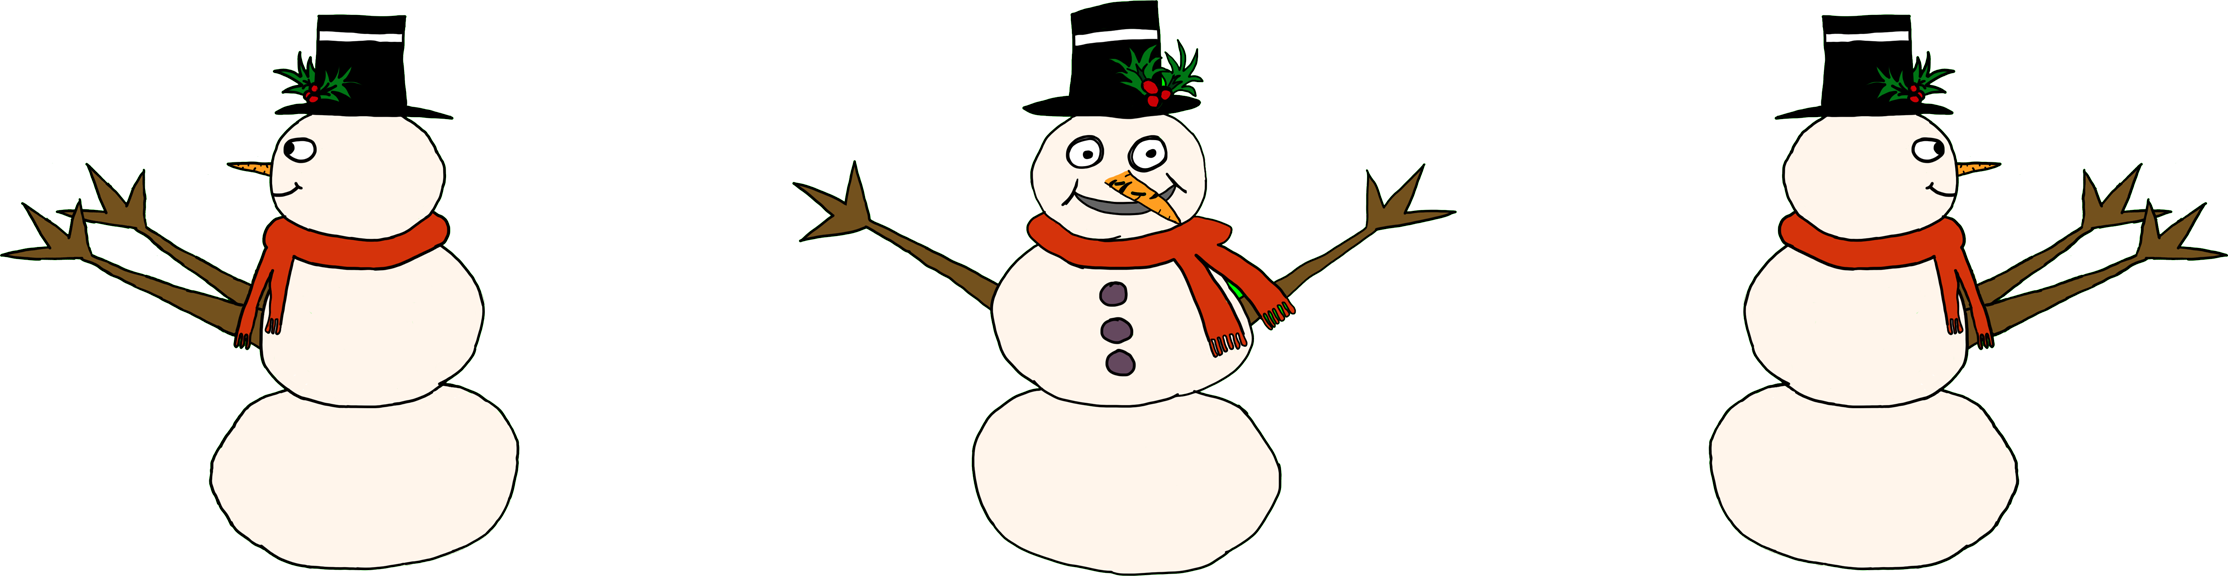
\includegraphics[width=1.00\textwidth]{Pictures/Design/SnowManShowOff.png}
\caption{Picture illustrating 3 different animations for one avatar}
\label{fig:Design_SnowmanAnimation}
\end{figure} 
\subsection{Sprite sheets}
There are many ways of animating an avatar for use on other platforms. One way is to finalize the animation on beforehand and play the actual footage. This is however not a very efficient way of including an animation as it take up space depending on the file format and size. Ultimately having several animations would slow down the program producing a vague output. Instead another solution was taken into considerations.\\
It was decided to create complete sprite sheets, to be implemented in Unity for use of animations. A sprite sheet contain all the images needed to create the full cycle and depending on the movement of the user in front of the installation on the library, the different sprite sheets will be activated. Figure \eqref{fig:Design_PixieBoyWalking} illustrates a complete sprite sheet for a user moving horizontally to the right.
\begin{figure}[htbp]
\centering
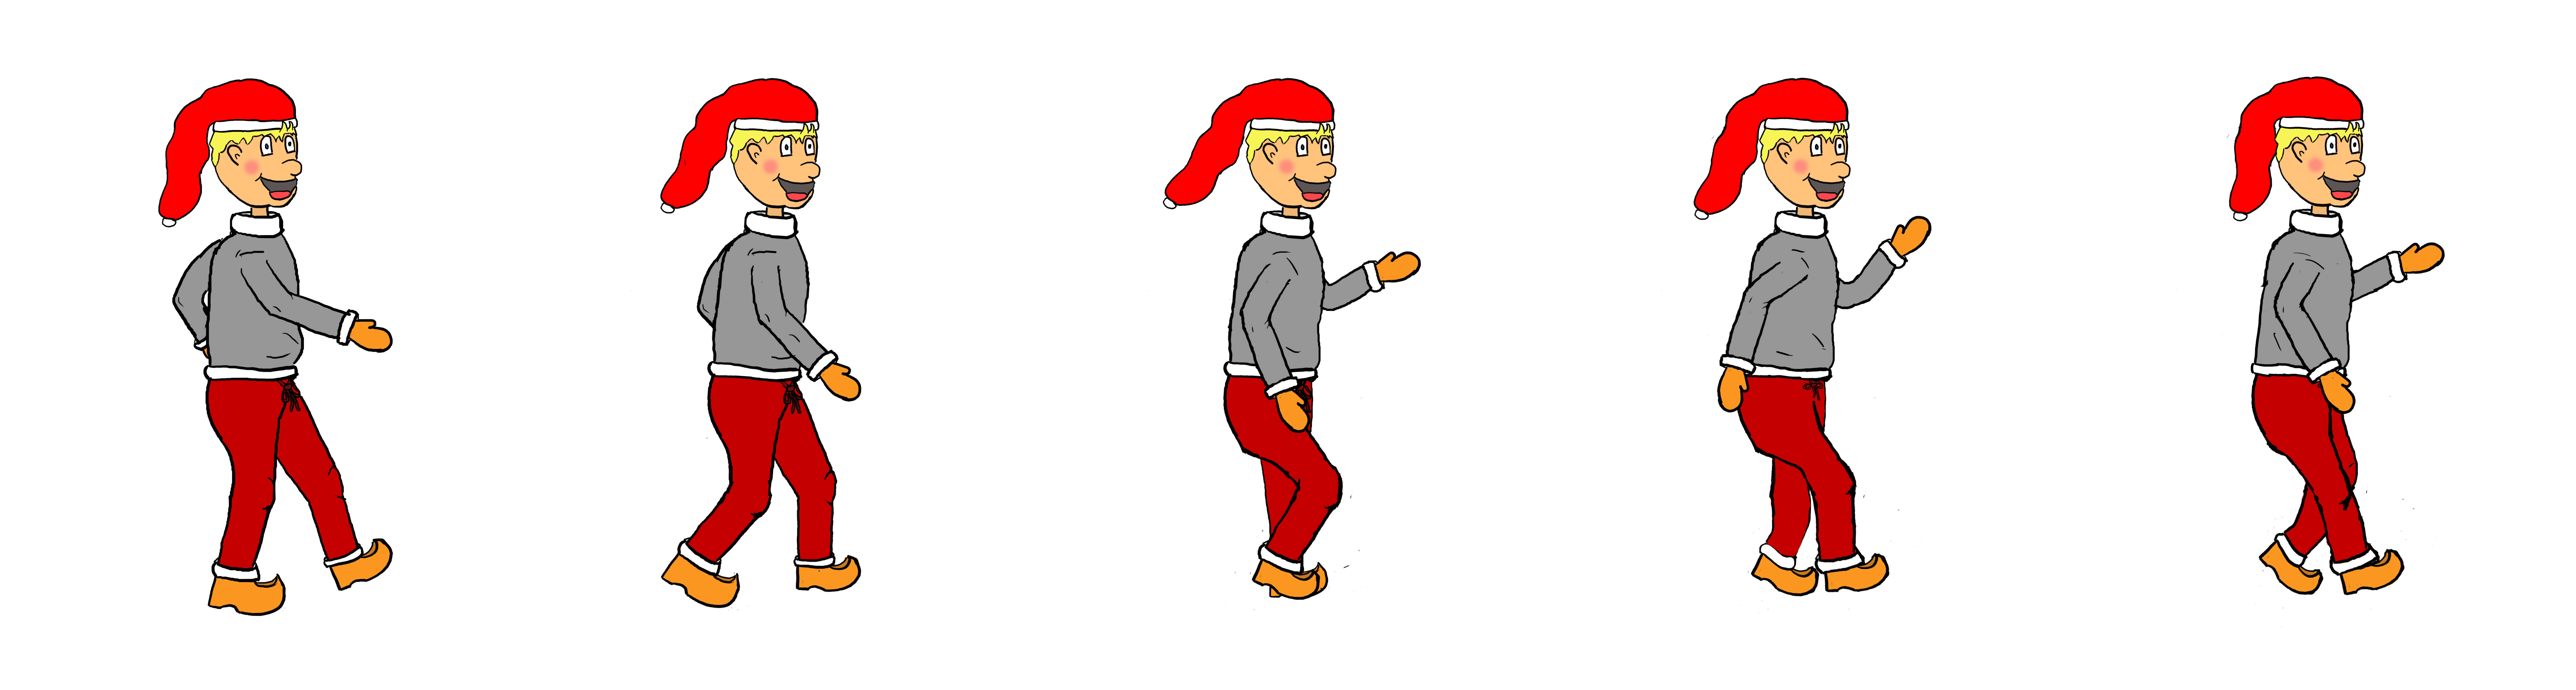
\includegraphics[width=1.00\textwidth]{Pictures/Design/PixieWalking.png}
\caption{Picture illustrating the walk cycle of the pixie boy}
\label{fig:Design_PixieBoyWalking}
\end{figure}